\chapter{Transversale pulse}
\fancyfoot[LO,RE]{Fisika: Golwe, klank en lig}
         

\section{Inleiding en sleutelkonsepte}
    \nopagebreak
    \label{m38801*cid2}
            %\subsection*{Inleiding}
            %\nopagebreak
Hierdie hoofstuk vorm die basis vir die bespreking van meganiese golwe in die opeenvolgende hoofstukke. Ons bespreek pulse eerste. Pulse is versteurings in 'n medium. As jy jou vinger in 'n emmer met water druk, sien jy 'n versteuring wat wegbeweeg van die punt waar jy aan die water geraak het. Die versteuring is 'n puls wat wegbeweeg van waar jy aan die water geraak het.
            

\subsection*{Wat is 'n \textsl{medium}?}
            \nopagebreak
\begin{minipage}{.5\textwidth}

 'n Medium is die materiaal waardeur 'n puls beweeg. Die medium dra die puls van een plek na 'n ander. Die medium skep nie die puls nie en is ook self nie die puls nie. Dus beweeg die medium nie saam met die puls soos dit deur die medium beweeg nie.

In elke medium beweeg die deeltjies wat die medium vorm \textit{tydelik} weg van hulle rusposisies. Vir 'n golf om voort te plant moet die verskillende dele van die medium in wisselwerking met mekaar wees.
\end{minipage}
\begin{minipage}{.5\textwidth}
\begin{center}
\textbf{ 'n Versteuring in water}\par
 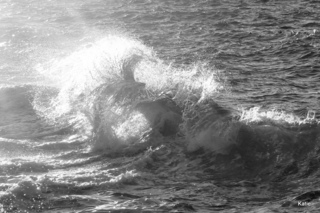
\includegraphics[width=.8\textwidth]{photos/waveby-mikeyskatie-flickr.jpg}\par
\textit{\small Beeld deur mikeyskatie on Flickr.com}
\end{center}
\end{minipage}


\label{m38801*fhsst!!!underscore!!!id51}

    \label{m38801*cid4}
\Definition{ Medium } {  'n Medium is die materiaal waardeur 'n puls beweeg.   } 
           
\section{Pulse: amplitude and lengte}

\subsection*{Wat is 'n \textsl{puls}?}
    \nopagebreak
    \begin{Investigation}{Observasie van pulse}

    \nopagebreak
    Vat 'n swaar tou. Kry twee mense om die tou horisontaal styf te trek. Wip die tou aan een kant.
    
    \begin{figure}[H]
	\nonumber
        \begin{center}
            \begin{pspicture}(-0.2,0)(5,1.4)
                \rput(0,0.8){\rope}
                \uput[d](2.5,0.8){Wip die tou aan een kant}
                \rput(-0.2,0){\psline{->}(0,0.6)(0,1.2)}
            \end{pspicture}
        \end{center}
    \end{figure}
    \par 
    Wat gebeur met die versteuring wat jy in die tou geskep het? Bly dit op die plek waar jy dit geskep het of beweeg dit deur die lengte van die tou?
    \end{Investigation}

In die ondersoek het ons `n \textsl{puls} geskep. 'n Puls is 'n \textsl{enkele} versteuring wat deur 'n medium beweeg. In 'n transversale puls is die versteuring van die medium loodreg op die rigting van die puls se beweging. Figuur~\ref{m38801*uid2!!!underscore!!!media} wys 'n voorbeeld van 'n transversale puls. In die ondersoek het ons 'n tou horisontaal gehou en die puls het die tou op en af maak beweeg. Dit is 'n voorbeeld van 'n transversale puls.\par

    \Definition{Puls}{'n Puls is 'n enkele versteuring wat deur 'n medium beweeg.} 

    \Definition{Transversale pulse }{'n Puls waar al die deeltjies wat versteur word deur die pulse loodreg (teen 'n regte hoek) op die rigting van die puls beweeg. } 
     
\subsubsection*{Pulslengte en amplitude}
\nopagebreak

Die amplitude van 'n puls is die hoeveelheid wat die medium tydelik verplaas word van sy rusposisie af. Die pulslengte is wys hoe lank die puls duur. Beide hierdie hoeveelhede word aangedui in Figuur~\ref{m38801*uid2!!!underscore!!!media}.
\par 

\Definition{Amplitude}{
Die amplitude van 'n puls is die afstand wat 'n medium vanuit sy rusposisie verplaas word.\\
Hoeveelheid: Amplitude (A) \hspace{.5cm} Eenheid naam: meter \hspace{.5cm} Eenheid simbool: $m$} 
\begin{figure}[h]
    \begin{center}
        \begin{pspicture}(0,-0.6)(5,2.2)
            \pnode(1,0){b}
            \pnode(2.5,0){c}
            \pnode(3.5,0){d}
            \pnode(5,0){e}
            \psline(b)(c)
            \rput(c){\psplot[xunit=0.034]{0}{30}{6 x mul sin 2 mul}}
            \psline(d)(e)
            \psline[linestyle=dotted]{<->}(2.4,0)(2.4,2)
            \uput[l](2.3,1){amplitude (A)}
            \psline[linestyle=dotted]{<->}(2.5,-0.1)(3.5,-0.1)
            \uput[d](3,0){puls lengte}
            \psline{->}(-0.3,0)(0.7,0)
            \uput[l](-0.3,0){Rusposisie}
        \end{pspicture}
    \end{center}
\caption{Voorbeeld van 'n transversale puls}
\label{m38801*uid2!!!underscore!!!media}
\end{figure}


Die rusposisie is die posisie wat die medium in is sonder enige versteurings. Dit word ook die ekwilibrium posisie genoem. Die woorde \textsl{rus} en \textsl{ekwilibrium} word dikwels afwisselend gebruik.

\begin{Investigation}{Pulslengte en amplitude}
\nopagebreak
Die grafieke hieronder dui die posisies van 'n puls by verskillende tye aan. \par
\begin{figure}[H]
\begin{center}
\begin{pspicture}(0,-4.2)(5,1.2)
\def\pulse{\psplot[xunit=0.017]{0}{30}{6 x mul sin}
\pcline{|-|}(0,0)(0,1)\uput[l](0,0.5){$A$}
\pcline[offset=-5pt]{|-|}(0,0)(0.5,0)\uput[d](0.25,-0.1){$p$}}
\rput(0,0){\pulse}\psline(0.5,0)(5,0)
\psline(0,-1.2)(1,-1.2)\rput(1,-1.2){\pulse}\psline(1.5,-1.2)(5,-1.2)
\psline(0,-2.4)(2,-2.4)\rput(2,-2.4){\pulse}\psline(2.5,-2.4)(5,-2.4)
\psline(0,-3.6)(3,-3.6)\rput(3,-3.6){\pulse}\psline(3.5,-3.6)(5,-3.6)
\uput[ur](5,0){$t$=0~s}
\uput[ur](5,-1.2){$t$=1~s}
\uput[ur](5,-2.4){$t$=2~s}
\uput[ur](5,-3.6){$t$=3~s}
\end{pspicture}
\end{center}
\end{figure}       
        \par
        Gebruik jou liniaal om die lengtes van $A$ en $p$ te meet. Skryf jou antwoorde in die tabel \par. 
          \begin{table}[H]
        \begin{center}
      \label{m38801*id313027}
      \tablelasttail{}
      \begin{xtabular}[t]{|l|l|l|}\hline
        Tyd &
                  $A$
                 &
                  $p$
                % make-rowspan-placeholders
     \tabularnewline\cline{1-1}\cline{2-2}\cline{3-3}
      %--------------------------------------------------------------------
        $t=0$~s &
         &
        % make-rowspan-placeholders
     \tabularnewline\cline{1-1}\cline{2-2}\cline{3-3}
      %--------------------------------------------------------------------
        $t=1$~s &
         &
        % make-rowspan-placeholders
     \tabularnewline\cline{1-1}\cline{2-2}\cline{3-3}
      %--------------------------------------------------------------------
        $t=2$~s &
         &
        % make-rowspan-placeholders
     \tabularnewline\cline{1-1}\cline{2-2}\cline{3-3}
      %--------------------------------------------------------------------
        $t=3$~s &
         &
        % make-rowspan-placeholders
     \tabularnewline\cline{1-1}\cline{2-2}\cline{3-3}
      %--------------------------------------------------------------------
    \end{xtabular}
      \end{center}
\end{table}
    \par
        Wat sien jy in die waardes van $A$ en $p$?
 \par 
In die ondersoek het ons gesien dat die amplitude ($A$) en die lengte ($p$) van 'n puls dieselfde is op verskillende tye is. \textsl{Pulslengte} en \textsl{amplitude} is twee belangrike groottes van 'n puls.
\end{Investigation}

\subsubsection*{Pulsspoed}
            \nopagebreak
\par
           \Definition{Pulsspoed } { \label{m38801*meaningfhsst!!!underscore!!!id145}
        \label{m38801*id313292}Pulsspoed is die afstand wat 'n puls in 'n eenheid tyd beweeg. \\
Hoeveelheid: Puls spoed ($v$) \hspace{.5cm} Eenheid naam: meter per sekond \hspace{.5cm} Eenheid simbool: $\text{m}\cdot \text{s}^{-1}$           } 
        
Spoed word gedefinieer as die afstand beweeg per eenheid tyd (hierdie word in meer detail bespreek in ``Beweging in een dimensie''). As die puls 'n afstand $D$ beweeg in 'n tyd $t$, is die spoed $v$:
        \label{m38801*uid4}\nopagebreak\noindent{}
    \begin{equation}
    \boxed{v=\frac{D}{t}}\nonumber
      \end{equation}
\par
            \label{m38801*secfhsst!!!underscore!!!id161}\vspace{.5cm} 
      \noindent



    \begin{wex}
    {%title
    Pulsspoed 
    }
    {%Question
        'n Puls beweeg $2m$ in $4s$ op 'n swaar tou. Bereken die spoed van die puls.
    }
    {% Answer
        \westep{Ontleed die vraag}{ 
        \label{m38801*id313393}Ons is gegee:\par 
        

        \label{m38801*id313396}
        \begin{itemize}[noitemsep]
            \item Die afstand wat die puls beweeg het: $D=2\phantom{\rule{2pt}{0ex}}\text{m}$
            \item Die tyd wat die puls geneem het om so ver te beweeg: $2\phantom{\rule{2pt}{0ex}}\text{m}$: $t=4\phantom{\rule{2pt}{0ex}}\text{s}$
        \end{itemize}
        
        \label{m38801*id313439}Ons moet die spoed van die puls bereken.\par 
        }
        
        \westep{Pas die beginsels toe}{
        \label{m38801*id313447}Ons kan:\par 
        \label{m38801*id313450}\nopagebreak\noindent{}
    \begin{equation}
    v=\frac{D}{t}\nonumber
    \end{equation}
        \label{m38801*id313470}gebruik om die spoed van die puls te bereken.\par }

    
        \westep{Doen die berekening}{  
        \label{m38801*id313479}\nopagebreak\noindent{}
    \begin{equation}\nonumber
    \begin{array}{ccc}\hfill v& =& \frac{D}{t}\hfill \\ & =& \frac{2\phantom{\rule{0.166667em}{0ex}}\text{m}}{4\phantom{\rule{0.166667em}{0ex}}\text{s}}\hfill \\ & =& 0,5\phantom{\rule{0.166667em}{0ex}}\text{m}\ensuremath{\cdot}{\text{s}}^{-1}\hfill \end{array}
      \end{equation}}

        \westep{Skryf die finale antwoord neer}{  
        \label{m38801*id313763}Die puls se spoed is $0,5\phantom{\rule{2pt}{0ex}}\text{m}\ensuremath{\cdot}\text{s}{}^{-1}$.
    } 
    }   
    \end{wex}


    \noindent
\label{m38801*notfhsst!!!underscore!!!id259}
      \Tip{Die puls se spoed is afhanklik van die eienskappe van die medium en nie die amplitude of lengte van die puls nie.}
 \begin{exercises}{Pulsspoed}
\noindent
\nopagebreak
\begin{enumerate}[noitemsep, label=\textbf{\arabic*}. ] 
\item 'n Puls beweeg $5\phantom{\rule{2pt}{0ex}}\text{m}$ in $15\phantom{\rule{2pt}{0ex}}\text{s}$. Bereken die spoed van die puls.\newline
\item 'n Puls het 'n spoed van $5\phantom{\rule{2pt}{0ex}}\text{cm}\ensuremath{\cdot}\text{s}{}^{-1}$. Hoe ver beweeg dit in $2,5\phantom{\rule{2pt}{0ex}}\text{s}$?\newline
\item 'n Puls het 'n spoed van $0,5\phantom{\rule{2pt}{0ex}}\text{m}\ensuremath{\cdot}\text{s}{}^{-1}$. Hoe lank sal dit neem om 'n afstand van $25\phantom{\rule{2pt}{0ex}}\text{cm}$ te bweeg?\newline
\label{m38801*uid10}\item Hoe lank sal dit neem vir 'n puls wat teen $0,25\phantom{\rule{2pt}{0ex}}\text{m}\ensuremath{\cdot}\text{s}{}^{-1}$ beweeg om 'n afstand van $20\phantom{\rule{2pt}{0ex}}\text{m}$ af te l\^{e}?\newline
\label{m38801*uid11}\item Die diagram wys twee pulse in dieselfde medium. Watter een het die ho\"{e}r spoed? Verduidelik jou antwoord.
\begin{figure}[H] % horizontal\label{m38801*id313945}
\begin{center}
\begin{pspicture*}(-0.6,-0.6)(4,1.8)
\psgrid[gridcolor=lightgray]
\psset{xunit=0.0055}
\rput(0,-0.4){\psplot{0}{180}{x sin 0.5 mul}\uput[l](0,0){A}\psline(180,0)(720,0)}
\rput(0,0.6){\psplot{0}{180}{x sin 1.1 mul}\uput[l](0,0){B}\psline(180,0)(720,0)}
\end{pspicture*}
\end{center}
\end{figure}               

\end{enumerate}
\label{m38801**end}
\practiceinfo
\par \begin{tabular}[h]{cccccc}
(1.) 02de  &  (2.) 02df  &  (3.) 02dg  &  (4.) 02dh  &  (5.) 02di  & \end{tabular}

\end{exercises}



\section{Superponering van pulse}

\mindsetvid{Superposition}{VPciu}
Twee of meer pulse kan terselfdertyd deur dieselfde medium beweeg. Wanneer dit gebeur reageer hulle met mekaar om 'n verskillende versteuring vorm op daardie punt. Die resultante puls word verkry deur die \textsl{beginsel van superponering}.

\Definition{Beginsel van superponering}{
Die beginsel van superposise s\^{e} wanneer twee versteurings terselfdertyd dieselfde spasie beset, dat die resultante versteuring die som van die twee versteurings is.}

Nadat die pulse deur mekaar beweeg het, beweeg elke puls op sy oorspronklike rigting en sy oorspronklike amplitude bly onveranderd. \par

Konstruktiewe interferensie vind plaas wanneer twee pulse mekaar ontmoet om 'n groter puls te skep. Die amplitude van die resultante puls is die som van die amplitudes van die twee oorspronklike pulse. Dit kan twee kruine of twee tr\^oe wees wat ontmoet. Hierdie effek word aangedui in Figuur \ref{m38802*uid53!!!underscore!!!media}.\par 

\Definition{ Konstruktiewe interferensie} {
     Konstruktiewe interferensie is wanneer twee pulse ontmoet om 'n groter puls te skep.
       } 
	
\begin{figure}[H] % horizontal\label{m38802*uid53}
\begin{center}
    \scalebox{0.7}
    {
    \begin{pspicture}(0,-5)(4,1.8)
    %\psgrid[gridcolor=lightgray]
    \def\pulse{\psline[linecolor=white,linestyle=solid,linewidth=2pt](0,0)(1.02,0)\psplot[xunit=0.034]{0}{30}{6 x mul sin}}
\psline(2.,1.2,)(2.,-5.)
    \rput(-3,0){\uput[u](2,1.2){pulse beweeg na mekaar toe}
    \psline(0,0)(4,0)
    \rput(0,0){\psline{->}(0,1.2)(0.5,1.2)\pulse}
    \psline{<-}(3.5,1.2)(4,1.2)\rput(3,0){\pulse}}

    \rput(-3,-3){\uput[u](2,2.2){pulse interfereer konstruktief}
    \psline(0,0)(4,0)
    \rput(1.5,0){\psset{yunit=2}\pulse}}

    \rput(-3,-5){\uput[u](2,1.2){pulse beweeg weg van mekaar}
    \psline(0,0)(4,0)
    \rput(0,0){\psline{<-}(0,1.2)(0.5,1.2)\pulse}
    \psline{->}(3.5,1.2)(4,1.2)\rput(3,0){\pulse}}
%     \end{pspicture}
%     }
% \end{minipage}
% \begin{minipage}{.5\textwidth}
%     \scalebox{0.7}
%     {
%     \begin{pspicture}(0,-5)(4,1.8)
%     %\psgrid[gridcolor=lightgray]
    \def\pulse{\psline[linecolor=white,linestyle=solid,linewidth=2pt](0,0)(1.02,0)\psplot[xunit=0.034]{0}{30}{-6 x mul sin}}

    \rput(3,0){\uput[u](2,1.2){pulse beweeg na mekaar toe}
    \psline(0,1)(4,1)
    \rput(0,1){\psline{->}(0,.2)(0.5,0.2)\pulse}
    \psline{<-}(3.5,1.2)(4,1.2)\rput(3,1){\pulse}}

    \rput(3,-3){\uput[u](2,2.2){pulse interfereer konstruktief}
    \psline(0,2)(4,2)
    \rput(1.5,2){\psset{yunit=2}\pulse}}

    \rput(3,-5){\uput[u](2,1.2){pulse beweeg weg van mekaar}
    \psline(0,1)(4,1)
    \rput(0,1){\psline{<-}(0,.2)(0.5,0.2)\pulse}
    \psline{->}(3.5,1.2)(4,1.2)\rput(3,1){\pulse}}
    \end{pspicture}
    }
\end{center}    
\caption{Superponering van twee pulse: konstruktiewe interferensie.}
\label{m38802*uid53!!!underscore!!!media}
 \end{figure}       



Destruktiewe interferensie vind plaas wanneer twee pulse mekaar ontmoet en 'n kleiner puls skep. Die amplitude van die resultante puls is die som van die amplitudes van die oorspronklike pulse, maar die een amplitude is 'n negatiewe getal. Dit word aangedui in Figuur \ref{m38802*uid54!!!underscore!!!media}. Amplitudes van individuele pulse word oor die algemeen gesom om die amplitude van die resultante puls te gee.\par 

\Definition{  Destruktiewe interferensie} { \label{m38802*meaningfhsst!!!underscore!!!id578}
Destruktiewe interferensie is wanneer twee pulse ontmoet om 'n kleiner puls te skep.
       } 
    

\begin{figure}[H] % horizontal\label{m38802*uid54}
    \begin{center}
    \scalebox{0.7}
    {
        \begin{pspicture}(0,-7)(10,1.8)
            %\psgrid[gridcolor=lightgray]
            \def\pulse{\psline[linecolor=white,linestyle=solid,linewidth=2pt](0,0)(1.02,0)\psplot[xunit=0.034]{0}{30}{6 x mul sin}}
            \def\dotpulse{\psplot[linestyle=dashed,xunit=0.034]{0}{30}{6 x mul sin}}
            \psline(5,1.2)(5,-6)
            \uput[u](2,1.2){pulse beweeg na mekaar toe}
            \psline(0,0)(4,0)
            \psline{->}(0,1.2)(0.5,1.2)
            \rput(0,0){\pulse}
            \psline{<-}(3.5,1.2)(4,1.2)
            \rput{180}(4,0){\pulse}

            \rput(0,-3){
            \uput[u](2,1.2){pulse interfereer destruktief}
            \psline(0,0)(4,0)
            \rput{180}(2.5,0){\dotpulse}
            \rput(1.5,0){\dotpulse}
            }

            \rput(0,-6){
            \uput[u](2,1.2){pulse beweeg weg van mekaar}
            \psline(0,0)(4,0)
            \psline{<-}(0,1.2)(0.5,1.2)
            \rput{180}(1,0){\pulse}
            \psline{->}(3.5,1.2)(4,1.2)
            \rput(3,0){\pulse}
            }
            %% second pic

            \uput[u](8,1.2){pulse beweeg na mekaar toe}
            \psline(6,-0.5)(10,-0.5)
            \psline{->}(6,1.1)(6.5,1.1)
            \rput(6,-0.5){\psset{yunit=1.5}\pulse}
            \psline{<-}(9.5,1.1)(10,1.1)
            \rput{180}(10,-0.5){\pulse}

            \rput(6,-3){\uput[u](2,0.6){pulse interfereer destruktief}
            \psline(0,0)(4,0)
            \rput(1.5,0){\psset{yunit=0.5}\pulse}}

            \rput(6,-6){
            \uput[u](2,1.6){pulse beweeg weg van mekaar}
            \psline(0,0)(4,0)
            \psline{<-}(0,1.6)(0.5,1.6)
            \rput{180}(1,0){\pulse}
            \psline{->}(3.5,1.6)(4,1.6)
            \rput(3,0){\psset{yunit=1.5}\pulse}}

        \end{pspicture}
    }
    \end{center}
\caption{Superponering van twee pulse. Die linkerkantste beelde demonstreer destruktiewe interferensie sedert die pulse mekaar kanseleer. Die regterkantste beelde dui gedeeltelike kansellasie want die pulse amplitudes is nie dieselfde nie.}
% \label{m38802*uid54!!!underscore!!!media}
 \end{figure}
\vspace{-1cm}
\begin{wex}{Superponering van pulse}{Die twee pulse hieronder aangedui beweeg na mekaar teen 1~\ms. Skets die golfvorm na 1~s, 2~s en 5~s.
\begin{center}
\begin{pspicture}(-1,-1)(8.6,2.6)
%\psgrid[gridcolor=lightgray]
\psaxes{<->}(0,0)(8.5,2.6)
\pcline[offset=0.4cm,linestyle=none](0,0)(0,2.6)
\aput{:U}{amplitude (m)}
\pcline[offset=-0.4cm,linestyle=none](0,0)(8.5,0)
\bput{:U}{afstand (m)}
\rput(2,0){\psline(0,0)(0,1)(1,1)(1,0)\pcline{->}(0.2,1.2)(0.8,1.2)\aput{:U}{A}}
\rput(6,0){\psline(0,0)(0,1)(1,1)(1,0)\pcline{<-}(0.2,1.2)(0.8,1.2)\aput{:U}{B}}
\end{pspicture}
\end{center}}{\westep{Na 1~s}
Na 1~$s$, puls A het 1 $m$ regs beweeg en puls B het 1 $m$ links beweeg
\begin{center}
\begin{pspicture}(-1,-1)(8.6,2.6)
%\psgrid[gridcolor=lightgray]
\psaxes{<->}(0,0)(8.5,2.6)
\pcline[offset=0.4cm,linestyle=none](0,0)(0,2.6)
\aput{:U}{amplitude (m)}
\pcline[offset=-0.4cm,linestyle=none](0,0)(8.5,0)
\bput{:U}{afstand (m)}
\rput(3,0){\psline(0,0)(0,1)(1,1)(1,0)\pcline{->}(0.2,1.2)(0.8,1.2)\aput{:U}{A}}
\rput(5,0){\psline(0,0)(0,1)(1,1)(1,0)\pcline{<-}(0.2,1.2)(0.8,1.2)\aput{:U}{B}}
\end{pspicture}
\end{center}

\westep{Na 2~s}
Na nog 1~$s$, puls A het nog 1 $m$ regs beweeg en puls B het 1 $m$ links beweeg
\begin{center}
\begin{pspicture}(-1,-1)(8.6,2.6)
%\psgrid[gridcolor=lightgray]
\psaxes{<->}(0,0)(8.5,2.6)
\pcline[offset=0.4cm,linestyle=none](0,0)(0,2.6)
\aput{:U}{amplitude (m)}
\pcline[offset=-0.4cm,linestyle=none](0,0)(8.5,0)
\bput{:U}{afstand (m)}
\rput(4,0){\psline(0,0)(0,2)(1,2)(1,0)\pcline[linestyle=none](0.2,2.2)(0.8,2.2)\aput{:U}{A+B}}
\end{pspicture}
\end{center}

\westep{Na 5~s}
Na 5~$s$, puls A het 5 $m$ regs beweeg en puls B het 5 $m$ links beweeg
\begin{center}
\begin{pspicture}(-1,-1)(8.6,2.6)
%\psgrid[gridcolor=lightgray]
\psaxes{<->}(0,0)(8.5,2.6)
\pcline[offset=0.4cm,linestyle=none](0,0)(0,2.6)
\aput{:U}{amplitude (m)}
\pcline[offset=-0.4cm,linestyle=none](0,0)(8.5,0)
\bput{:U}{afstand (m)}
\rput(7,0){\psline(0,0)(0,1)(1,1)(1,0)\pcline{->}(0.2,1.2)(0.8,1.2)\aput{:U}{A}}
\rput(1,0){\psline(0,0)(0,1)(1,1)(1,0)\pcline{<-}(0.2,1.2)(0.8,1.2)\aput{:U}{B}}
\end{pspicture}
\end{center}}\end{wex}
    
%    \noindent
%\label{m38802*notfhsst!!!underscore!!!id635}
%\Tip{The idea of superponering is one that occurs often in physics. You will see \textsl{much, much more} of superponering!}
\vspace{-1cm}
\label{m38802*eip-791}
\begin{g_experiment}{Konstruktiewe en destruktiewe interferensie} \nopagebreak
\textbf{Doel}
Om konstruktiewe en destruktiewe interferensie te demonstreer\\
\label{m38802*eip7241}\noindent{}\textbf{Apparaat} 
Golftenk apparaat	
\begin{figure}[H] % horizontal\label{m38802*id63458}
    \begin{center}
    \label{m38802*id63458!!!underscore!!!media}\label{m38802*id63458!!!underscore!!!printimage}\includegraphics[width=0.8\columnwidth]{col11305.imgs/m38802_rippletray.png} % m38802;rippletray.png;;;6.0;8.5;
%       \vspace{2pt}
%     \vspace{.1in}
    \end{center}
 \end{figure}  
\textbf{Metode}
\begin{enumerate}[noitemsep, label=\textbf{\arabic*}. ] 
    \item Stel die golftenk op
    \item Maak 'n enkele puls (jy kan enige manier gebruik om dit te doen, tik die water met jou vinger of laat val 'n druppel in die water) en kyk wat gebeur of laat val 'n druppel in die water)
    \item Maak twee pulse gelyktydig en kyk wat gebeur.
    \item Maak twee pulse op verskillende tye en kyk wat gebeur.
\end{enumerate}     
\textbf{Resultate en gevolgtrekkings}
Jy behoort te sien dat wanneer jy twee pulse gelyktydig opwek hulle konstruktief interfereer en wanneer hulle op verskillende tye opgewek word interfereer hulle destruktief. 
\end{g_experiment}

\begin{exercises}{Probleme wat superponering van pulse behels.}
            \nopagebreak \vspace{-1.5cm}
            \label{m38802*id316401}\begin{enumerate}[noitemsep, label=\textbf{\arabic*}. ] 
\item Vir die volgende pulse, skets die resultante golfvorms na $1\phantom{\rule{2pt}{0ex}}\text{s}$, $2\phantom{\rule{2pt}{0ex}}\text{s}$, $3\phantom{\rule{2pt}{0ex}}\text{s}$, $4\phantom{\rule{2pt}{0ex}}\text{s}$ and $5\phantom{\rule{2pt}{0ex}}\text{s}$. Elke puls beweeg teen $1\phantom{\rule{2pt}{0ex}}\text{m}\ensuremath{\cdot}\text{s}{}^{-1}$. Elke blok verteenwoordig $1\phantom{\rule{2pt}{0ex}}\text{m}$. Die pulse word aangedui as dik swart lyne en die onverplaasde medium as strepieslyne. 
\begin{figure}[H] % horizontal\label{m38802*id316460}
\begin{center}
\begin{pspicture}(-0.5,-1.4)(10,1.4)
\rput{90}(-0.5){Amplitude (m)}
\rput[r](-0.05,0){0}
\rput[r](-0.05,1){1}
\rput[l](1.0,-.15){1}
\rput[l](2.0,-.15){2}
\rput[l](3.0,-.15){3}
\rput[l](4.0,-.15){4}
\rput[l](5.0,-.15){5}
\rput[l](6.0,-.15){6}
\rput[l](7.0,-.15){7}
\rput[l](8.0,-.15){8}
\rput[l](9.0,-.15){9}
\rput(8.5,-1.3){Posisie (m)}
\psgrid[gridcolor=lightgray,gridlabels=0,subgriddiv=1](0,-1)(10,1)
\psline[linestyle=dashed](0,0)(2,0)(2,1)(4,1)(4,0)(6,0)(6,1)(8,1)(8,0)(10,0)
\psline[linewidth=0.08cm](2,0)(2,1)(4,1)(4,0)
\psline[linewidth=0.08cm](6,0)(6,1)(8,1)(8,0)
\psline{->}(2,1.2)(2.5,1.2)
\psline{<-}(7.5,1.2)(8,1.2)
\uput[ur](0,0.4){$t$=0~s}
\end{pspicture}
\end{center}
\end{figure}    

\item Vir die volgende pulse, skets die resultante golfvorms na $1\phantom{\rule{2pt}{0ex}}\text{s}$, $2\phantom{\rule{2pt}{0ex}}\text{s}$, $3\phantom{\rule{2pt}{0ex}}\text{s}$, $4\phantom{\rule{2pt}{0ex}}\text{s}$ and $5\phantom{\rule{2pt}{0ex}}\text{s}$. Elke puls beweeg teen $1\phantom{\rule{2pt}{0ex}}\text{m}\ensuremath{\cdot}\text{s}{}^{-1}$. Elke blok verteenwoordig $1\phantom{\rule{2pt}{0ex}}\text{m}$. Die pulse word aangedui as dik swart lyne en die onverplaasde medium as strepieslyne. 
\begin{figure}[H] % horizontal\label{m38802*id316477}
\begin{center}
\begin{pspicture}(-0.5,-1.4)(10,1.4)
\rput{90}(-0.5){Amplitude (m)}
\rput[r](-0.05,0){0}
\rput[r](-0.05,1){1}
\rput[l](1.0,-.15){1}
\rput[l](2.0,-.15){2}
\rput[l](3.0,-.15){3}
\rput[l](4.0,-.15){4}
\rput[l](5.0,-.15){5}
\rput[l](6.0,-.15){6}
\rput[l](7.0,-.15){7}
\rput[l](8.0,-.15){8}
\rput[l](9.0,-.15){9}
\rput(8.5,-1.3){Posisie (m)}
\psgrid[gridcolor=lightgray,gridlabels=0,subgriddiv=1](0,-1)(10,1)
\psline[linestyle=dashed](0,0)(2,0)(2,1)(4,1)(4,0)(6,0)(6,-1)(8,-1)(8,0)(10,0)
\psline[linewidth=0.08cm](2,0)(2,1)(4,1)(4,0)
\psline[linewidth=0.08cm](6,0)(6,-1)(8,-1)(8,0)
\psline{->}(2,1.2)(2.5,1.2)
\psline{<-}(7.5,1.2)(8,1.2)
\uput[ur](0,0.4){$t$=0~s}
\end{pspicture}
\end{center}
\end{figure} 

\item Vir die volgende pulse, skets die resultante golfvorms na $1\phantom{\rule{2pt}{0ex}}\text{s}$, $2\phantom{\rule{2pt}{0ex}}\text{s}$, $3\phantom{\rule{2pt}{0ex}}\text{s}$, $4\phantom{\rule{2pt}{0ex}}\text{s}$ and $5\phantom{\rule{2pt}{0ex}}\text{s}$. Elke puls beweeg teen $1\phantom{\rule{2pt}{0ex}}\text{m}\ensuremath{\cdot}\text{s}{}^{-1}$. Elke blok verteenwoordig $1\phantom{\rule{2pt}{0ex}}\text{m}$. Die pulse word aangedui as dik swart lyne en die onverplaasde medium as strepieslyne. 
    \setcounter{subfigure}{0}
\begin{figure}[H] % horizontal\label{m38802*id316495}
\begin{center}
\begin{pspicture}(-0.5,-1.4)(10,1.4)
\rput{90}(-0.5){Amplitude (m)}
\rput[r](-0.05,0){0}
\rput[r](-0.05,1){1}
\rput[l](1.0,-.15){1}
\rput[l](2.0,-.15){2}
\rput[l](3.0,-.15){3}
\rput[l](4.0,-.15){4}
\rput[l](5.0,-.15){5}
\rput[l](6.0,-.15){6}
\rput[l](7.0,-.15){7}
\rput[l](8.0,-.15){8}
\rput[l](9.0,-.15){9}
\rput(8.5,-1.3){Posisie (m)}
\psgrid[gridcolor=lightgray,gridlabels=0,subgriddiv=1](0,-1)(10,1)
\psline[linestyle=dashed](0,0)(2,0)(2,1)(3,1)(3,-1)(4,-1)(4,0)(6,0)(6,-1)(7,-1)(7,1)(8,1)(8,0)(10,0)
\psline[linewidth=0.08cm](2,0)(2,1)(3,1)(3,-1)(4,-1)(4,0)
\psline[linewidth=0.08cm](6,0)(6,-1)(7,-1)(7,1)(8,1)(8,0)
\psline{->}(2,1.2)(2.5,1.2)
\psline{<-}(7.5,1.2)(8,1.2)
\uput[ur](0,0.4){$t$=0~s}
\end{pspicture}
\end{center}
\end{figure}


\item Vir die volgende pulse, skets die resultante golfvorms na $1\phantom{\rule{2pt}{0ex}}\text{s}$, $2\phantom{\rule{2pt}{0ex}}\text{s}$, $3\phantom{\rule{2pt}{0ex}}\text{s}$, $4\phantom{\rule{2pt}{0ex}}\text{s}$ and $5\phantom{\rule{2pt}{0ex}}\text{s}$. Elke puls beweeg teen $1\phantom{\rule{2pt}{0ex}}\text{m}\ensuremath{\cdot}\text{s}{}^{-1}$. Elke blok verteenwoordig $1\phantom{\rule{2pt}{0ex}}\text{m}$. Die pulse word aangedui as dik swart lyne en die onverplaasde medium as strepieslyne. 
    \setcounter{subfigure}{0}
\begin{figure}[H] % horizontal\label{m38802*id316512}
\begin{center}
\begin{pspicture}(-0.5,-1.4)(10,1.4)
\rput{90}(-0.5){Amplitude (m)}
\rput[r](-0.05,0){0}
\rput[r](-0.05,1){1}
\rput[l](1.0,-.15){1}
\rput[l](2.0,-.15){2}
\rput[l](3.0,-.15){3}
\rput[l](4.0,-.15){4}
\rput[l](5.0,-.15){5}
\rput[l](6.0,-.15){6}
\rput[l](7.0,-.15){7}
\rput[l](8.0,-.15){8}
\rput[l](9.0,-.15){9}
\rput(8.5,-1.3){Posisie (m)}
\psgrid[gridcolor=lightgray,gridlabels=0,subgriddiv=1](0,-1)(10,1)
\psline[linestyle=dashed](0,0)(2,0)(2,1)(3,1)(3,-1)(4,-1)(4,0)(6,0)(6,1)(7,1)(7,-1)(8,-1)(8,0)(10,0)
\psline[linewidth=0.08cm](2,0)(2,1)(3,1)(3,-1)(4,-1)(4,0)
\psline[linewidth=0.08cm](6,0)(6,1)(7,1)(7,-1)(8,-1)(8,0)
\psline{->}(2,1.2)(2.5,1.2)
\psline{<-}(7.5,1.2)(8,1.2)
\uput[ur](0,0.4){$t$=0~s}
\end{pspicture}
\end{center}
\end{figure}

\item Vir die volgende pulse, skets die resultante golfvorms na $1\phantom{\rule{2pt}{0ex}}\text{s}$, $2\phantom{\rule{2pt}{0ex}}\text{s}$, $3\phantom{\rule{2pt}{0ex}}\text{s}$, $4\phantom{\rule{2pt}{0ex}}\text{s}$ and $5\phantom{\rule{2pt}{0ex}}\text{s}$. Elke puls beweeg teen $1\phantom{\rule{2pt}{0ex}}\text{m}\ensuremath{\cdot}\text{s}{}^{-1}$. Elke blok verteenwoordig $1\phantom{\rule{2pt}{0ex}}\text{m}$. Die pulse word aangedui as dik swart lyne en die onverplaasde medium as strepieslyne. 
    \setcounter{subfigure}{0}
\begin{figure}[H] % horizontal\label{m38802*id316530}
\begin{center}
\begin{pspicture}(-0.5,-1.4)(10,1.4)
\rput{90}(-0.5){Amplitude (m)}
\rput[r](-0.05,0){0}
\rput[r](-0.05,1){1}
\rput[l](1.0,-.15){1}
\rput[l](2.0,-.15){2}
\rput[l](3.0,-.15){3}
\rput[l](4.0,-.15){4}
\rput[l](5.0,-.15){5}
\rput[l](6.0,-.15){6}
\rput[l](7.0,-.15){7}
\rput[l](8.0,-.15){8}
\rput[l](9.0,-.15){9}
\rput(8.5,-1.3){Posisie (m)}
\psgrid[gridcolor=lightgray,gridlabels=0,subgriddiv=1](0,-1)(10,1)
\psline[linestyle=dashed](0,0)(2,0)(2,1)(5,1)(5,0)(7,0)(7,1)(8,1)(8,0)(10,0)
\psline[linewidth=0.08cm](2,0)(2,1)(5,1)(5,0)
\psline[linewidth=0.08cm](7,0)(7,1)(8,1)(8,0)
\psline{->}(2,1.2)(2.5,1.2)
\psline{<-}(7.5,1.2)(8,1.2)
\uput[ur](0,0.4){$t$=0~s}
\end{pspicture}
\end{center}
\end{figure}    


\item Vir die volgende pulse, skets die resultante golfvorms na $1\phantom{\rule{2pt}{0ex}}\text{s}$, $2\phantom{\rule{2pt}{0ex}}\text{s}$, $3\phantom{\rule{2pt}{0ex}}\text{s}$, $4\phantom{\rule{2pt}{0ex}}\text{s}$ and $5\phantom{\rule{2pt}{0ex}}\text{s}$. Elke puls beweeg teen $1\phantom{\rule{2pt}{0ex}}\text{m}\ensuremath{\cdot}\text{s}{}^{-1}$. Elke blok verteenwoordig $1\phantom{\rule{2pt}{0ex}}\text{m}$. Die pulse word aangedui as dik swart lyne en die onverplaasde medium as strepieslyne. 
    \setcounter{subfigure}{0}
\begin{figure}[H] % horizontal\label{m38802*id316547}
\begin{center}
\begin{pspicture}(-0.5,-1.4)(10,1.4)
\rput{90}(-0.5){Amplitude (m)}
\rput[r](-0.05,0){0}
\rput[r](-0.05,1){1}
\rput[l](1.0,-.15){1}
\rput[l](2.0,-.15){2}
\rput[l](3.0,-.15){3}
\rput[l](4.0,-.15){4}
\rput[l](5.0,-.15){5}
\rput[l](6.0,-.15){6}
\rput[l](7.0,-.15){7}
\rput[l](8.0,-.15){8}
\rput[l](9.0,-.15){9}
\rput(8.5,-1.3){Posisie (m)}
\psgrid[gridcolor=lightgray,gridlabels=0,subgriddiv=1](0,-1)(10,1)
\psline[linestyle=dashed](0,0)(2,0)(2,1)(5,1)(5,0)(7,0)(7,-1)(8,-1)(8,0)(10,0)
\psline[linewidth=0.08cm](2,0)(2,1)(5,1)(5,0)
\psline[linewidth=0.08cm](7,0)(7,-1)(8,-1)(8,0)
\psline{->}(2,1.2)(2.5,1.2)
\psline{<-}(7.5,1.2)(8,1.2)
\uput[ur](0,0.4){$t$=0~s}
\end{pspicture}
\end{center}
\end{figure}              

 \label{m38802*uid62}\item Wat is superponering van golwe?\newline
\label{m38802*uid64}\item Wat is konstruktiewe interferensie?\newline
\label{m38802*uid65}\item Wat is destruktiewe interferensie?\newline
        \end{enumerate}
% \label{m38802*fs-id1165499443114} The following presentation provides a summary of the work covered in this chapter. Although the presentation is titled waves, the presentation covers pulses only.
%     \setcounter{subfigure}{0}
% 	\begin{figure}[H] % horizontal\label{m38802*slidesharefigure}
%     \label{m38802*slidesharemedia}\label{m38802*slideshareflash}\raisebox{-5 pt}{ \includegraphics[width=0.5cm]{col11305.imgs/summary_www.png}} { (Presentation:  P10039 )}
%  \end{figure}       

\practiceinfo
 \begin{tabular}[h]{cccccc}
 (1.) 02dj  &  (2.) 02dk  &  (3.) 02dm  &  (4.) 02dn  &  (5.) 02dp  &  (6.) 02dq  &  (7.) 02dr  &  (8.) 02ds  &  (9.) 02dt  & \end{tabular}

\end{exercises}
%\pagebreak
            \summary{VPcjo}
            \nopagebreak
            \label{m38802*eip-404}\begin{itemize}[noitemsep]
            \item 'n Medium is die materiaal waarin 'n puls beweeg.
	    \item 'n Puls is die enkele versteuring wat deur 'n medium beweeg. 
	    \item Die amplitude is die meting van hoe ver die medium vanuit sy rusposisie verplaas word. 
	    \item Pulsspoed is die afstand wat 'n puls in een eenheid tyd beweeg.
	    \item Konstruktiewe interferensie is wanneer twee pulse mekaar ontmoet en 'n groter puls skep.
	    \item Destruktiewe interferensie is wanneer twee pulse mekaar ontmoet en 'n kleiner puls skep.
	    \end{itemize}
        \label{m38802*cid9}
\begin{table}[H]
\begin{center}
\begin{tabular}{|l|c|c|}\hline \hline 
\multicolumn{3}{|c|}{\textbf{Fisiese Hoeveelhede}}\\ \hline \hline
\multicolumn{1}{|c|}{\textbf{Hoeveelheid}} & \textbf{Eenheid naam} & \textbf{Eenheid simbool}\\ \hline
Amplitude ($A$) & meter & m \\ \hline
Pulse spoed ($v$) & meter per sekond & $\text{m} \cdot \text{s}^{-1}$ \\ \hline
\end{tabular}
\end{center}
\caption{Eenhede wat gebruik word met \textbf{transversale pulse}  }
\label{table:electrostatics::units}
\end{table}
% \begin{table}[H]
% \begin{center}
% \begin{tabular}{|l|c|c|c|}\hline \hline 
% \multicolumn{4}{|c|}{\textbf{Eenhede}}\\ \hline \hline
% \textbf{Hoeveelheid} & \textbf{Simbool} & \textbf{Eenheid} & \textbf{S.I. Eenheid}  \\ \hline
% Amplitude & $A$ & \multicolumn{2}{c|}{m} \\ \hline
% Pulse spoed & $v$ & \multicolumn{2}{c|}{$\text{m} \cdot \text{s}^{-1}$} \\ \hline
% \end{tabular}
% \end{center}
% \caption{Eenhede wat gebruik word met \textbf{transversale pulse} }
% \label{table:electricity::units}
% \end{table}
\vspace{-1cm}
\begin{eocexercises}{Transversale pulse}
            \nopagebreak \vspace{-1cm}
      \label{m38802*id316647}\begin{enumerate}[noitemsep, label=\textbf{\arabic*}. ] 
            \label{m38802*uid66}\item 'n Swaar tou word opwaards gewip om 'n enkele puls in die tou te skep. Maak 'n skets van die tou en dui die volgende daarop aan:
\label{m38802*id316663}\begin{enumerate}[noitemsep, label=\textbf{\alph*}. ] 
\item Die rigting waarin die puls beweeg.
\item Amplitude
\item Pulslengte
\item Rusposisie
\end{enumerate}

\item 'n Puls het 'n spoed van $2,5\phantom{\rule{2pt}{0ex}}\text{m}\ensuremath{\cdot}\text{s}{}^{-1}$. Hoe ver sal dit beweeg in $6\phantom{\rule{2pt}{0ex}}\text{s}$?\newline
\item 'n Puls beweeg 'n afstand van $75\phantom{\rule{2pt}{0ex}}\text{cm}$ in $2,5\phantom{\rule{2pt}{0ex}}\text{s}$ af. Wat is die spoed van die puls?\newline
\item Hoe lank sal dit 'n puls neem om 'n afstand van $200\phantom{\rule{2pt}{0ex}}\text{mm}$ af te l\^{e} as sy spoed $4\phantom{\rule{2pt}{0ex}}\text{m}\ensuremath{\cdot}\text{s}{}^{-1}$ is?\newline

%                 \label{m38802*uid82}\item Two pulses, A and B, of identical shape and amplitude are simultaneously generated in two identical wires of equal mass and length. Wire A is, however, pulled tighter than wire B. Which pulse will arrive at the other end first, or will they both arrive at the same time?\newline
\end{enumerate}
\vspace{-1cm}
\practiceinfo
 \begin{tabular}[h]{ccccc}
 (1.) 02du  &  (2.) 02dv  &  (3.) 02dw  &  (4.) 02dx  &   \end{tabular}
\end{eocexercises}
